\begin{appendices}
  \section{Proofs for Section 3}

\begin{proof}[Proof of Theorem \ref{thm: weighted}]
By the strong law of large numbers, we have the almost sure convergence for the estimator
\begin{align*}
    \hat{\mu}_{W}(a) &=  \frac{\frac{1}{N}\sum_{i = 1}^N \pr(A_i = a \mid Z_i)Y_i}{\frac{1}{N}\sum_{i = 1}^N \pr(A_i = a \mid Z_i)} \\
    &\overset{\text{a.s.}}{\to} \frac{\expect [\pr (A = a \mid Z)Y]}{\expect [\pr (A = a \mid Z)]} \\
    &= \frac{\expect [\expect (\ind (A = a) \mid Z) \expect (Y \mid Z)]}{\pr (A = a)}.
\end{align*}
For the true mean group outcome, introduce the trivial conditional expectation with respect to $Z$:
\begin{align*}
    \mu(a) = \frac{\expect[\ind (A = a)Y]}{\pr (A = a)} = \frac{\expect [\expect (\ind (A = a)Y \mid Z)]}{\pr (A = a)}
\end{align*}
Thus, we can regroup the terms in the difference to recognize the conditional covariance
\begin{align*}
    &\hat{\mu}_{W}(a) - \mu(a) \\
    \overset{\text{a.s.}}{\to} &-\frac{\expect [\expect (\ind (A = a)Y \mid Z) - \expect (\ind (A = a) \mid Z) \expect(Y \mid Z)]}{\pr (A = a)} \\
    = & -\frac{\expect [\cov (\ind(A = a), Y \mid Z)]}{\pr (A = a)}.
\end{align*}
The analogous results hold for $A=b$ everywhere.
\end{proof}

\begin{proof}[Proof of Corollary \ref{corr:weighted-unbiased}]
When $Y$ is independent of $A$ conditionally on $Z$, it immediately follows that
\[
\cov (\ind(A = a), Y \mid Z) = \cov (\ind(A = b), Y \mid Z) = 0,
\]
and thus
\begin{align*}
    \hat{\mu}_{W}(a) - \mu(a) &\overset{\text{a.s.}}{\to} 0\\
    \hat{\mu}_{W}(b) - \mu(b) &\overset{\text{a.s.}}{\to} 0 \\
\therefore \hat{\delta}_{W} - \delta &\overset{\text{a.s.}}{\to} 0
\end{align*}
\end{proof}

\begin{proof}[Proof of Theorem \ref{thm: demographic-est-race-bias}]
Define the following events for $u_1, u_2 \in \{a, b\}$:
\begin{align*}
 \mathcal{E}_q^+(u_1, u_2) &= \{\pr (A = u_1 \mid Z) > q, A = u_2\} \\
 \mathcal{E}_q^-(u_1, u_2) &= \{ \pr (A = u_1 \mid Z) \le q, A = u_2\}.
\end{align*}
Then
\begin{align*}
    \{A = a\} &= \mathcal{E}_q^+(a, a) \cup \mathcal{E}_q^-(a, a), \\
    \{\hat{A} = a\} &= \mathcal{E}_q^+(a, a) \cup \mathcal{E}_q^+(a, b),
\end{align*}
where $\hat{A}$ is the estimated protected attribute according to the thresholding rule (Definition \ref{def:thresholding_rule}).

It follows that
\begin{align*}
    \mu(a) &= \frac{\expect [\ind (A = a)Y]}{\pr(A = a)} \\
    &= \frac{\expect [\ind (\mathcal{E}_q^+(a, a))Y] + \expect [\ind (\mathcal{E}_q^-(a, a))Y]}{\pr(\mathcal{E}_q^+(a, a)) + \pr(\mathcal{E}_q^-(a, a))} \\
    \hat{\mu}_W(a) &\overset{\text{a.s.}}{\to} \frac{\expect [\ind (\hat{A} = a)Y]}{\pr(\hat{A} = a)}  \\
    &= \frac{\expect [\ind (\mathcal{E}_q^+(a, a))Y] + \expect [\ind (\mathcal{E}_q^+(a, b))Y]}{\pr(\mathcal{E}_q^+(a, a)) + \pr(\mathcal{E}_q^+(a, b))}.
\end{align*}

Then simple algebra shows that
\begin{align*}
    \hat{\mu}_W(a) - \mu(a) &\overset{\text{a.s.}}{\to} \Delta_1(a)C_1(a) - \Delta_2(a)C_2(a) \\
    &+ (\Delta_1(a) - \Delta_2(a))C_3(a),
\end{align*}
where
\begin{align*}
    \Delta_1(a) = \expect[Y \mid \mathcal{E}_q^+(a, b)] - \expect[Y \mid \mathcal{E}_q^+(a, a)], \\
    \Delta_2(a) = \expect[Y \mid \mathcal{E}_q^-(a, a)] - \expect[Y \mid \mathcal{E}_q^+(a, a)],
\end{align*}
and
\begin{align*}
    C_1(a) = \pr(\hat{A} = a \mid A = a)\pr(A = b \mid \hat{A} = a), \\
    C_2(a) = \pr(A = a \mid \hat{A} = a)\pr(\hat{A} \ne a \mid A = a), \\
    C_3(a) = \pr(\hat{A} \ne a \mid A = a)\pr(A = b \mid \hat{A} = a).
\end{align*}
Similarly, we can prove that
\begin{align*}
    \hat{\mu}_W(b) - \mu(b) &\overset{\text{a.s.}}{\to} \Delta_1(b)C_1(b) - \Delta_2(b)C_2(b) \\
    &+ (\Delta_1(b) - \Delta_2(b))C_3(b),
\end{align*}
where $\Delta_1(b)$, $\Delta_2(b)$, $C_1(b)$, $C_2(b)$, $C_3(b)$ are defined analogously.

In summary, as ${N \to \infty}$, for $u \in \{a, b\}$ and $u^c$ as the class opposite to $u$, ,
\begin{align*}
    \hat{\mu}_{q}(u) - \mu(u) \to &\;\Delta_1(u)C_1(u) - \Delta_2(u)C_2(u) \\
    &+ (\Delta_1(u) - \Delta_2(u))C_3(u),
\end{align*}
where $\Delta_1(u)$ and $\Delta_2(u)$ are defined in Section 3.2, and

\begin{align*}
    C_1(u) &= \pr(\hat{A} = u \mid A = u)\pr(A = u^c \mid \hat{A} = u), \\
    C_2(u) &= \pr(A = u \mid \hat{A} = u)\pr(\hat{A} \ne u \mid A = u), \\
    C_3(u) &= \pr(\hat{A} \ne u \mid A = u)\pr(A = u^c \mid \hat{A} = u).
\end{align*}
% In the above formulas, $\{\hat{A} \ne u\} = \{\hat{A} = u^c\} \cup \{\hat{A} = \text{NA}\}$.


% Obviously $C_1(u), C_2(u), C_3(u) \in [0, 1]$ and
% \[
% C_1(u) + C_2(u) + C_3(u) = 1 - \pr({A} = u \mid \hat{A} = u)\pr(\hat{A} = u \mid {A} = u) \le 1.
% \]

\end{proof}


\begin{proof}[Proof of Corollary \ref{corollary: demographic-est-race}]
The conclusions follow immediately from Theorem \ref{thm: demographic-est-race-bias}.
\end{proof}

\begin{proof}[Proof of Corollary \ref{corollary: C-functions}]
First, (i) is obvious according to the formulas of $C_2(u), C_3(u)$ in Theorem \ref{thm: demographic-est-race-bias}.

Second, note that
\begin{align*}
C_1(u) &= \pr(\hat{A} = u \mid A = u)(1 - \pr(A = u \mid \hat{A} = u)), \\
C_2(u) &= \pr(A = u \mid \hat{A} = u)(1 - \pr(\hat{A} = u \mid A = u)).
\end{align*}

Thus
\begin{align*}
C_2(u) - C_1(u) &= \pr(A = u \mid \hat{A} = u) - \pr(\hat{A} = u \mid A = u) \\
                &= \pr(A = u, \hat{A} = u)[\frac{1}{\pr (\hat{A} = u)} - \frac{1}{\pr ({A} = u)}] \\
                &= \frac{\pr(A = u, \hat{A} = u)}{\pr (\hat{A} = u) \pr ({A} = u)}
                (\pr ({A} = u) - \pr (\hat{A} = u)).
\end{align*}

Therefore, $\pr (\hat{A} = u) < \pr ({A} = u)$ if and only if
\[
C_2(u) > C_1(u).
\]



\end{proof}

% \begin{proof}[Proof of Theorem \ref{thm: relation-weighted-thresholding}]
% We prove that if $\cov (\ind(A = a), Y \mid Z = z) < 0$ and $\cov (\ind(A = b), Y \mid Z = z) > 0$ for any $z$, then $\Delta_1(a) > 0$ in the following part and all other conclusions can be proved analogously.

% First, note that
% \begin{align*}
%     \cov (\ind(A = a), Y \mid Z = z) &= \expect [\ind (A = a)Y \mid Z = z] \\
%     &- \expect [\ind (A = a) \mid Z = z]\expect[Y \mid Z = z] \\
%     &= \expect[Y \mid A = a, Z = z]\pr (A = a \mid Z = z) \\
%     &- \expect[Y \mid Z = z]\pr (A = a \mid Z = z) < 0
% \end{align*}
% is equivalent to
% \[
% \expect[Y \mid A = a, Z = z] < \expect[Y \mid Z = z].
% \]
% Analogously, $\cov (\ind(A = b), Y \mid Z = z) > 0$ is equivalent to
% \[
% \expect[Y \mid A = b, Z = z] > \expect[Y \mid Z = z].
% \]
% Thus $\cov (\ind(A = a), Y \mid Z = z) < 0$ and $\cov (\ind(A = b), Y \mid Z = z) > 0$ imply that $\expect[Y \mid A = b, Z = z] > \expect[Y \mid A = a, Z = z]$.

% Second,
% \begin{align*}
%     & \qquad \qquad \expect [Y \mid \pr (A = a \mid Z) > q, A = a] \\
%     &= \frac{\sum_{z: \pr(A = a\mid Z = z) > q}\expect[Y \mid A = a, Z = z]\pr(Z = z\mid A = a)}{\pr (\pr (A = a \mid Z) > q \mid A = a)} \\
%     &= \frac{\sum_{z: \pr(A = a\mid Z = z) > q}\expect[Y \mid A = a, Z = z]\pr(Z = z\mid A = a)}{\pr (\hat{A} =  \mid A = a)} \\
%     & \qquad \qquad \expect [Y \mid \pr (A = a \mid Z) > q, A = b] \\
%     &= \frac{\sum_{z: \pr(A = a\mid Z = z) > q}\expect[Y \mid A = b, Z = z]\pr(Z = z\mid A = b)}{\pr (\pr (A = a \mid Z) > q \mid A = b)}\\
%     &= \frac{\sum_{z: \pr(A = a\mid Z = z) > q}\expect[Y \mid A = b, Z = z]\pr(Z = z\mid A = b)}{\pr (\hat{A} = a \mid A = b)}
% \end{align*}
% Given that

% \end{proof}



\section{Multilevel unknown protected class}
In this section, we suppose that the protected class $A$ can have more than two values and the value space of $A$ is denoted as $\mathcal{A}$. Denote $\mathcal{A}' = \mathcal{A}\backslash\{a, b\}$, i.e., $\mathcal{A}'$ is the set of all values of $A$ other than $a$ and $b$.


\begin{corollary} \label{corollary: C-functions-multiclass}
The quantities $C_1(u), C_2(u), C_3(u)$ for $u \in \{a, b\}$ in Theorem \ref{thm: demographic-est-race-bias} are related in the following way:
\begin{enumerate}[label=(\roman*)]
    \item If $\pr (A = u \mid \hat{A} = u) > \pr (A = u^c \mid \hat{A} = u)$, then $C_2(u) > C_3(u)$
    % \item If $\pr (\hat{A} = u \mid A = u) > \pr (\hat{A} \ne u \mid A = u)$, then $C_1(u) > C_3(u)$;
    \item If $\pr (A = u) + \pr (A \in \mathcal{A}', \hat{A} = u)> \pr (\hat{A} = u)$, then $C_2(u) > C_1(u)$.
\end{enumerate}
Thus if the conditions in (i) and (ii) both hold, then $C_2(u) > C_1(u)$ and $C_2(u) > C_3(u)$.
\end{corollary}

This means in the multiclass case, $C_2(u) > C_1(u)$ can hold more easily: it can hold even if $\pr (A = u) < \pr (\hat{A} = u)$, which explains why in figure \ref{figure: C_values} $C_2(u) > C_1(u)$ even though $\pr (A = u) < \pr (\hat{A} = u)$ where $u$ stands for White.  

% \begin{proof}

% \end{proof}

\section{Additional results on the mortgage dataset}
\subsection{Bias According to Theorem \ref{thm: demographic-est-race-bias}}\label{section:theory_bias}
\begin{figure}[H]
  \centering
    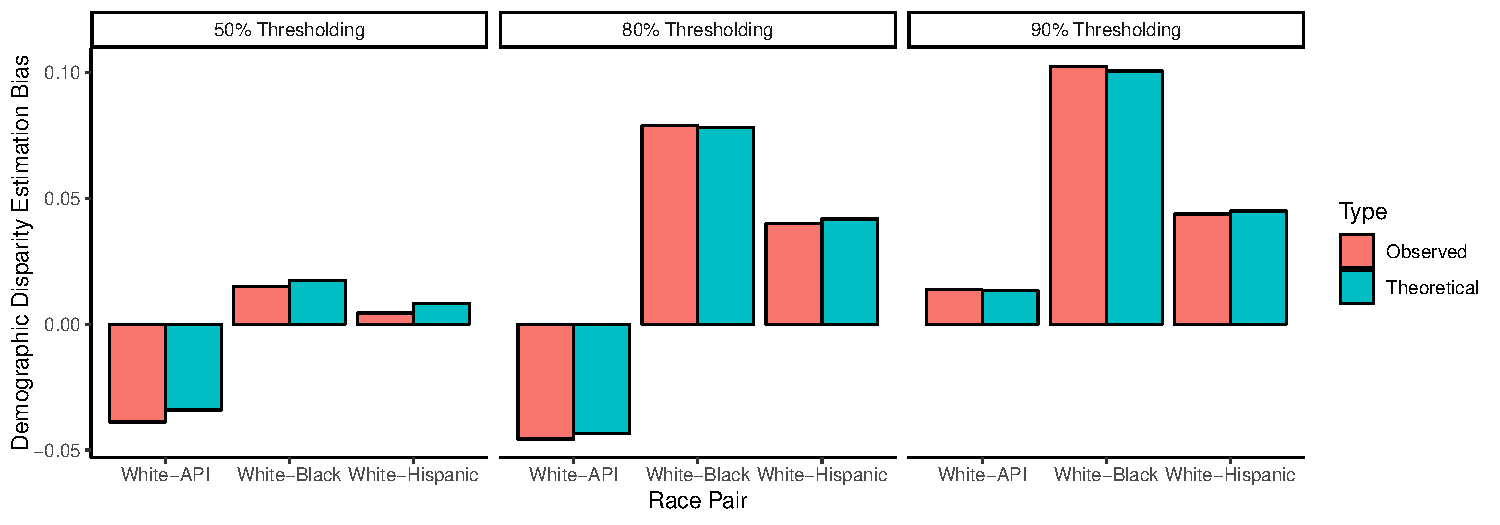
\includegraphics[width=\linewidth]{Theory_bias.pdf}
  \caption{The observed bias is the actual estimation bias of the thresholded estimators with different thresholds, as shown in the right subfigure of Figure \ref{figure: mortgage_demo_disparity}. The theoretical bias is computed according to Theorem \ref{thm: demographic-est-race-bias}. This figure shows that the theoretical bias formula in Theorem \ref{thm: demographic-est-race-bias} for binary protected class approximates the observed bias for multiclass protected class very well. Therefore, Theorem \ref{thm: demographic-est-race-bias} indeed captures the main bias sources of thresholded estimators for both binary and multiclass protected class.} \label{figure: theory_bias}
\end{figure}

\subsection{Results for API}
\begin{figure}[H]
  \centering
    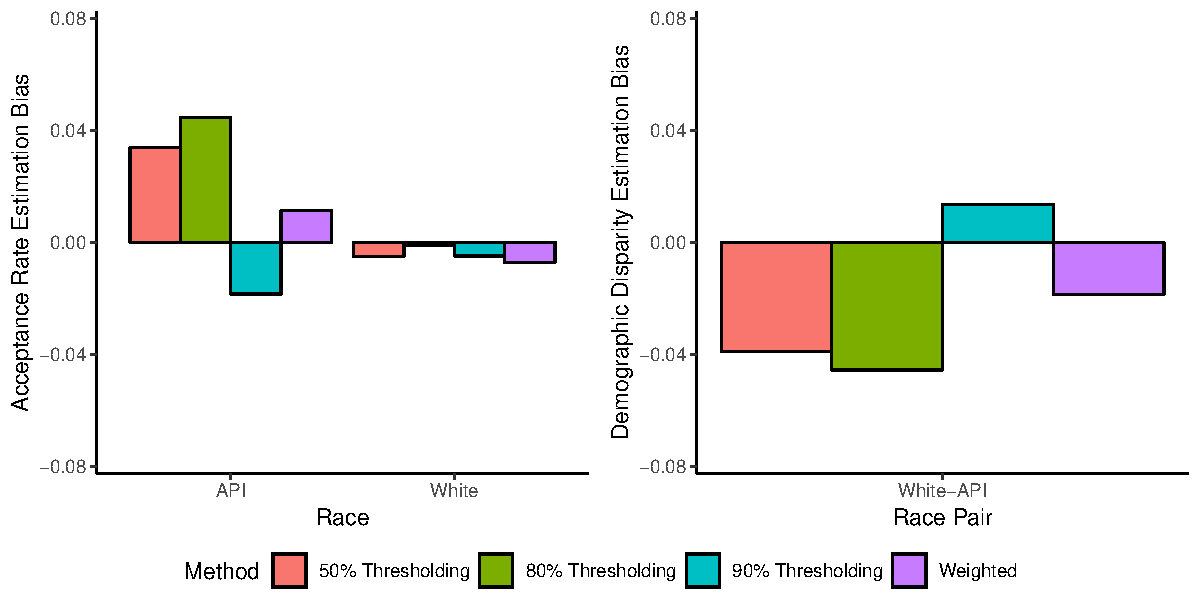
\includegraphics[width=\linewidth]{Demo_disparity_api.pdf}
  \caption{Left figure: the acceptance rate estimation bias for the API race. Right figure: demographic disparity estimation bias with respect to White and API.} \label{figure: mortgage_demo_api}
\end{figure}


\begin{figure}[H]
  \centering
    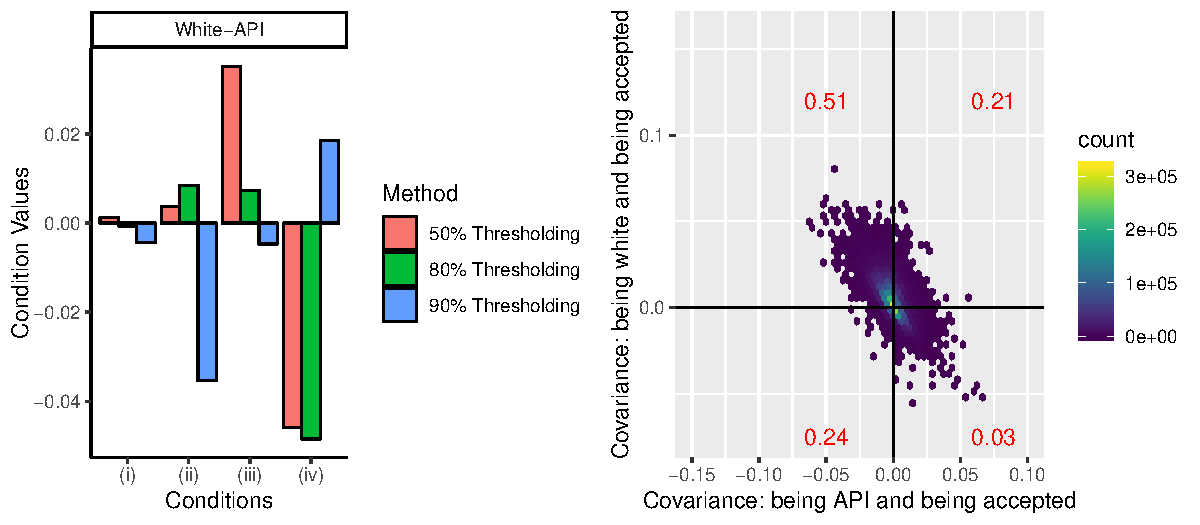
\includegraphics[width=\linewidth]{Condition_weighted_api.pdf}
  \caption{Left figure: the left hand side quantities in conditions \ref{eq:condition1}---\ref{eq:condition4} in Corollary \ref{corollary: demographic-est-race} when using thresholded estimator to estimate the demographic disparity with respect to White and API. Right figure: the population distribution across census tracts with different combinations of covariance terms in Theorem \ref{thm: weighted} with White as the advantaged group and API as the disadvantaged group.} \label{figure: condition_api}
\end{figure}

In Figure \ref{figure: mortgage_demo_api}, we can observe that the estimation bias is quite different when estimating the demographic disparity for White and API. The thresholded estimator could overestimate or underestimate the demographic disparity while the weighted estimator only very slightly underestimate the demographic disparity. This is not totally surprising because the API population have very different geolocation distribution and socioeconomic status distribution than Hispanic and Black. API population tend to mix with other races in terms of living locations and the average socioeconomic status disparity between API and White is much smaller than the average socioeconomic status disparity between other minority groups and White. Figure \ref{figure: condition_api} shows that the proportion of people who live in census tracts where API are accepted at lower average rate while White are accepted at higher average rate is much smaller than the proportion of people who live in census tracts where Black or Hispanic are accepted at lower average rate while White are accepted at higher average rate. This explains why the underestimation bias of the weighted estimator is very small.

\subsection{Correlation between the race probability and socioeconomic status}\label{section:correlation_income}
\begin{figure}[H]
  \centering
    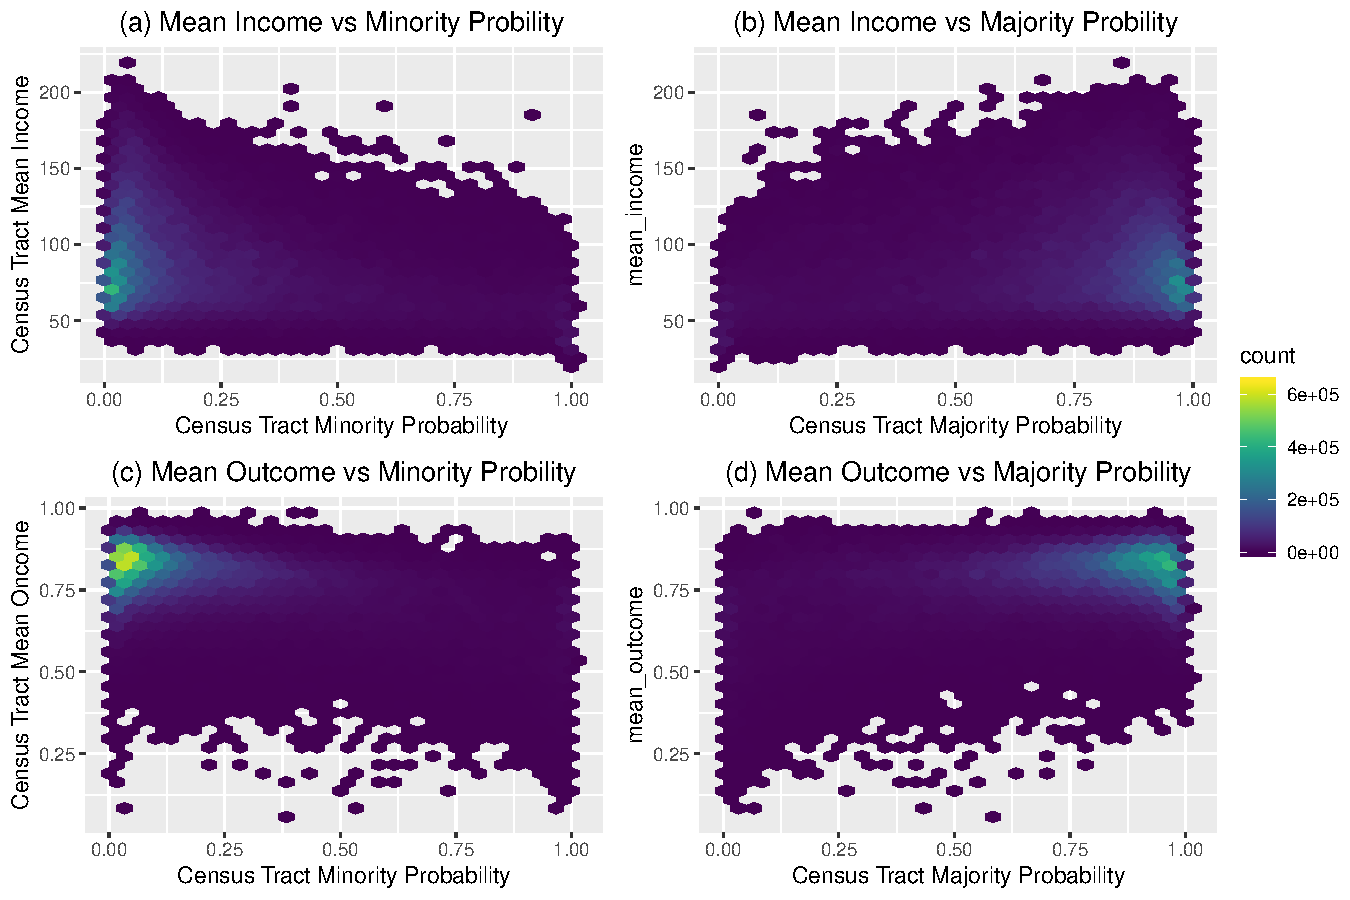
\includegraphics[width=\linewidth]{Income_prob_correlation.pdf}
  \caption{Figure (a) and (b) show the population distribution across census tracts with different mean yearly income versus different probability of belonging to the majority group and different probability of belonging to the minority groups. Figure (c) and (d) show the population distribution across census tracts with different average loan acceptance rate versus different probability of belonging to the majority group and different probability of belonging to the minority groups. The majority group here refers to White and the minority groups here refer to Black or Hispanic. } \label{figure: income_correlation}
\end{figure}

Figure \ref{figure: income_correlation} shows the correlation between the the race proxy probabilities and yearly income or average loan acceptance rate. We can clearly observe that census tracts with high White probability overall have more mass on higher income and higher loan acceptance rate while census tracts with high Hispanic or Black probability have more mass on lower income and lower loan acceptance rate. This figure validates the fact that the geolocation encodes socioeconomic status disparities such that the race proxy probabilities are correlated with socioeconomic status variables (e.g., income in this example) and the loan approval outcome. These correlations account for the conditions \eqref{eq:condition3}---\eqref{eq:condition4} in the Corollary \ref{corollary: demographic-est-race}.


\subsection{An example of unbiased weighted estimator} \label{section: unbiased_weighted}
\begin{figure}
  \centering
    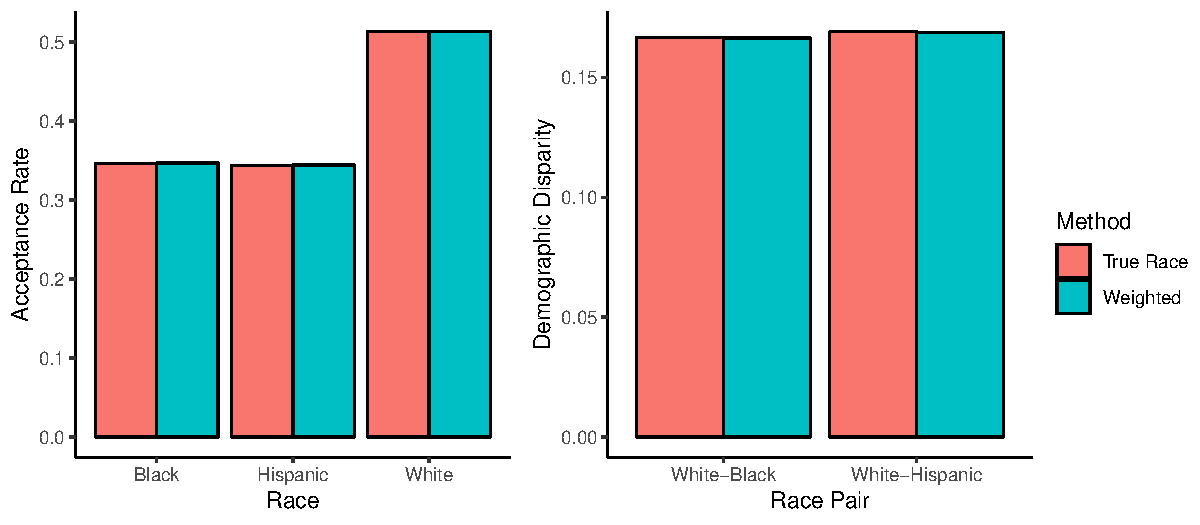
\includegraphics[width=\linewidth]{weighted_unbiased.pdf}
  \caption{The loan acceptance rate and demographic disparity estimated by using the true race and by the weighted estimator for the semi-synthetic data where income is used to estimate race and it also determines the loan outcome. Weighted estimator is unbiased in this case because race is independent with the outcome conditionally on income by construction.} \label{figure: weighted_unbiased}
\end{figure}

To provide an example where the weighted estimator can be unbiased, we construct a semi-synthetic dataset based on the mortgage dataset. We aggregate the mortgage applicants' yearly income into deciles and use this discrete income as the predictor for race. We simulate the loan approval outcome $Y$ with $\pr (Y = 1 \mid Z = z) = 1/(1 + \exp(-(z - 5.5)))$, i.e., the loan approval outcome only depends on the discrete income $Z$. By construction, the loan approval outcome $Y$ is independent with race $A$ conditionally on $Z$, thus according to Theorem \ref{thm: weighted} the weighted estimator should be unbiased. This theoretical result is verified in Figure \ref{figure: weighted_unbiased}. This example shows that the weighted estimator with well constructed proxy model can estimate the demographic disparity perfectly.

\end{appendices}
